\chapter{Probl\`emes d'int\'egration des \'equations du mouvement}

\section{Mouvement lin\'eaire}

\subsection{Oscillations d'un pendule math\'ematique plan}

\begin{figure}[htb!]
	\begin{center}
		\begin{picture}(100,100)(0,0)
			%axis
			\linethickness{0.05mm}
			\multiput(0,100)(10,0){10}{\line(1,0){8}}\put(102,95){$x$}
			\multiput(0,0)(0,10){10}{\line(0,1){8}}\put(-5,-10){$y$}
			%socle
			\put(0,100){\color{black}\circle*{5}}
			%arms
			\linethickness{0.5mm}
			\put(0,100){\line(10,-15){70}}
			\put(40,50){$l$}
			\put(68,-5){\color{black}\circle*{10}}\put(75,-7){$m$}
			%angles
			\linethickness{0.05mm}
			\qbezier(0,80),(5,82),(10,85)
			\put(3,70){$\varphi$}
		\end{picture}
		\caption{Pendule double oscillant}\label{FIG:3_1_1}
	\end{center}
\end{figure}

Il s'agit de trouver la p\'eriode d'oscillation du pendule en fonction de l'amplitude du mouvement. En supposant $\varphi_{0}$ l'angle maximal par rapport \`a la verticale, o\`u la vitesse du pendule est nulle, l'\'energie totale du pendule est :
\bea
	E & = & \frac{m}{2}\left[\dfrac{\mathrm{d}(l\varphi)}{\mathrm{dt}}\right]^{2} - mgl\cos\varphi \nonumber \\
	& = & \frac{m}{2}l^{2}\dot{\varphi}^{2} - mgl\cos\varphi
\eea
et par conservation de l'\'energie totale :
\be
	E = E(\varphi_{0}) = -mgl\cos\varphi_{0}
\ee
Par sym\'etrie du mouvement, la p\'eriode est \'egale au temps de parcours entre $\varphi=0$ et $\varphi=\varphi_{0}$. Sachant que la quantit\'e, $E-U$ vaut $-mgl\cos\varphi_{0} + mgl\cos\varphi$, l'\'equation (\ref{EQ:11_3}) peut s'\'ecrire :
\bea
	\mathrm{T} & = & 4\sqrt{\frac{m}{2}}\int_{0}^{\varphi_{0}}{\dfrac{\mathrm{d}(l\varphi)}{\sqrt{mgl(\cos\varphi - \cos\varphi_{0})}}} \nonumber \\
	& = & 4\sqrt{\frac{l}{2g}}\int_{0}^{\varphi_{0}}{\dfrac{\mathrm{d}\varphi}{\sqrt{\cos\varphi - \cos\varphi_{0}}}}
\eea
Notons que :
\bea
	\sin^{2}\frac{\alpha}{2} & = & \left(\dfrac{e^{i\frac{\alpha}{2}} - e^{-i\frac{\alpha}{2}}}{2i}\right)^{2} \nonumber \\
	& = & -\frac{1}{4}\left(e^{i\alpha} + e^{-i\alpha} - 2e^{i\frac{\alpha}{2}-i\frac{\alpha}{2}}\right) \nonumber \\
	& = & -\frac{1}{4}\left(e^{i\alpha} + e^{-i\alpha} - 2\right) \nonumber \\
	& = & \frac{1}{2}\left(1-\cos\alpha\right) \nonumber \\
	\Leftrightarrow \cos\alpha & = & 1 - 2\sin^{2}\frac{\alpha}{2}
\eea
Cela permet de d\'evelopper la p\'eriode telle que :
\bea
	\mathrm{T} & = & 4\sqrt{\frac{l}{2g}}\int_{0}^{\varphi_{0}}{\dfrac{\mathrm{d}\varphi}{\sqrt{1-2\sin\frac{\varphi}{2} - 1 + \sin\frac{\varphi_{0}}{2}}}} \nonumber \\
	& = & 4\sqrt{\frac{l}{2g}}\int_{0}^{\varphi_{0}}{\dfrac{\mathrm{d}\varphi}{\sqrt{2\left(\sin\frac{\varphi_{0}}{2} - \sin\frac{\varphi}{2}\right)}}} \nonumber \\
	& = & 2\sqrt{\frac{l}{g}}\int_{0}^{\varphi_{0}}{\dfrac{\mathrm{d}\varphi}{\sqrt{\sin\frac{\varphi_{0}}{2} - \sin\frac{\varphi}{2}}}}
\eea
En posant $\sin\xi = \dfrac{\sin(\varphi/2)}{\sin(\varphi_{0}/2)}$, nous avons pour $\varphi = 0$, $\sin\xi = 0$ soit $\xi = 0$ et pour $\varphi = \varphi_{0}$, $\sin\xi = 1$ soit $\xi = \frac{\pi}{2}$. En d\'eveloppant la d\'efinition de $\sin\xi$ pour l'inverser, nous trouvons :
\bea
	\sin^{2}\xi\sin^{2}\left(\frac{\varphi_{0}}{2}\right) & = & \sin^{2}\left(\frac{\varphi}{2}\right) \nonumber \\
	& = & 1 - \cos^{2}\left(\frac{\varphi}{2}\right) \nonumber \\
	\Leftrightarrow \cos\left(\frac{\varphi}{2}\right) & = & \sqrt{1 - \sin^{2}\left(\frac{\varphi_{0}}{2}\right)\sin^{2}\xi}
\eea
et pour conna\^itre la correspondance entre $\mathrm{d}\varphi$ et $\mathrm{d}\xi$ :
\bea
	\sin\xi & = & \dfrac{\sin\left(\frac{\varphi}{2}\right)}{\sin\left(\frac{\varphi_{0}}{2}\right)} \nonumber \\
	\Leftrightarrow \cos\xi\mathrm{d}\xi & = & \dfrac{\cos\left(\frac{\varphi}{2}\right)}{2\sin\left(\frac{\varphi_{0}}{2}\right)}\mathrm{d}\varphi \nonumber \\
	\mathrm{d}\varphi & = & \dfrac{2\sin\left(\frac{\varphi_{0}}{2}\right)\cos\xi}{\cos\left(\frac{\varphi}{2}\right)}\mathrm{d}\xi \nonumber \\
	& = & \dfrac{2\sin\left(\frac{\varphi_{0}}{2}\right)\sqrt{1 - \sin^{2}\xi}}{\cos\left(\frac{\varphi}{2}\right)}\mathrm{d}\xi \nonumber \\
	& = & \dfrac{2\sin\left(\frac{\varphi_{0}}{2}\right)\sqrt{1 - \dfrac{\sin^{2}\left(\frac{\varphi}{2}\right)}{\sin^{2}\left(\frac{\varphi_{0}}{2}\right)}}}{\cos\left(\frac{\varphi}{2}\right)}\mathrm{d}\xi \nonumber \\
	& = & \dfrac{2\sqrt{\sin^{2}\left(\frac{\varphi_{0}}{2}\right) - \sin^{2}\left(\frac{\varphi}{2}\right)}}{\cos\left(\frac{\varphi}{2}\right)}\mathrm{d}\xi \nonumber \\
	\Leftrightarrow \dfrac{\mathrm{d}\varphi}{\sqrt{\sin^{2}\left(\frac{\varphi_{0}}{2}\right) - \sin^{2}\left(\frac{\varphi}{2}\right)}} & = & \dfrac{2\mathrm{d}\xi}{\sqrt{1 - \sin^{2}\left(\frac{\varphi_{0}}{2}\right)\sin^{2}\xi}}
\eea
En cons\'equence, en posant :
\be
	K(k) = \int_{0}^{\frac{\pi}{2}}\dfrac{\mathrm{d}\xi}{\sqrt{1 - k^{2}\sin^{2}\xi}}
\ee
la p\'eriode $\mathrm{T}$ se r\'e\'ecrit ainsi\footnote{Dans le livre, il est indiqu\'e que l'argument de la fonction $K$ est $\frac{\sin\left(\varphi_{0}\right)}{2}$, je pense qu'il ne s'agit que d'une coquille.} :
\be
	\mathrm{T} = 4\sqrt{\dfrac{l}{g}}K\left(\sin(\varphi_{0}/2)\right)
\ee
La fonction $K$ est l'int\'egrale elliptique compl\`ete de premi\`ere esp\`ece. Elle admet comme d\'eveloppement en s\'erie enti\`ere :
\bea
	K(k) & = & \dfrac{\pi}{2}\sum_{n=0}^{+\infty}\left[\dfrac{(2n)!}{2^{2n}(n!)^{2}}\right]^{2}k^{2n} \nonumber \\
	& =& \dfrac{\pi}{2}\left(1 + \left(\dfrac{2}{4 \times 1}\right)^{2}k^{2} + \cdots\right)
\eea
donc pour de petites oscillations telles que $\sin(\varphi_{0}/2)\simeq\varphi_{0}/2\ll 1$ :
\be
	K(\sin\varphi_{0}/2) = \dfrac{\pi}{2}\left(1 + \dfrac{1}{16}\varphi_{0}^{2} + \cdots\right)
\ee
soit :
\be
	\mathrm{T} = 2\pi\sqrt{\dfrac{l}{g}}\left(1 + \dfrac{1}{16}\varphi_{0}^{2} + \cdots\right)
\ee
et en premi\`ere approximation, la p\'eriode du mouvement n'est d\'ependante ni de la masse de la particule ni de l'amplitude initiale.

\subsection{Cas d'\'energies potentielles particuli\`eres}

Il s'agit de d\'eterminer la p\'eriode d'oscillations en fonction de l'\'energie pour le mouvement d'une particule de masse $m$ dans un champ o\`u l'\'energie potentielle $U$ est d\'efinie telle que :

\subsubsection{$U = A\lvert x \rvert^{n}$}

\begin{figure}[htb!]
	\begin{center}
		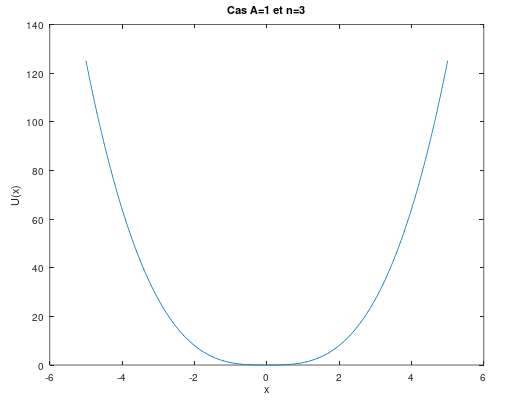
\includegraphics[width=10cm]{chapter_03_exercice_2a}
		\caption{$U = \lvert x \rvert^{n}$ pour $n \in \{1,2,3,4,5\}$}\label{FIG:3_2_a}
	\end{center}
\end{figure}

Dans ce cas pr\'ecis, commençons par d\'efinir les points d'arr\^et tels que $E=U$, soit $x = \pm\left(\dfrac{E}{A}\right)^{\frac{1}{n}}$. Cela permet d'\'ecrire l'\'equation (\ref{EQ:11_5}) telle que :
\bea
	\mathrm{T}(E) & = & \sqrt{2m}\int_{-\left(\frac{E}{A}\right)^{\frac{1}{n}}}^{+\left(\frac{E}{A}\right)^{\frac{1}{n}}}\dfrac{\mathrm{d}x}{\sqrt{E - A\lvert x \rvert^{n}}} \nonumber \\
	& = & 2\sqrt{2m}\int_{0}^{+\left(\frac{E}{A}\right)^{\frac{1}{n}}}\dfrac{\mathrm{d}x}{\sqrt{E - Ax^{n}}} \nonumber \\
	& = & 2\sqrt{\dfrac{2m}{E}}\int_{0}^{+\left(\frac{E}{A}\right)^{\frac{1}{n}}}\dfrac{\mathrm{d}x}{\sqrt{1 - \dfrac{Ax^{n}}{E}}}
\eea
car la fonction $U$ est paire, i.e. $U(x) = U(-x)$. En posant :
\be
	y = \left(\dfrac{A}{E}\right)^{\frac{1}{n}}x
\ee
qui permet d'\'ecrire :
\be
	\begin{cases}
		y^{n} = \dfrac{A}{E}x^{n} \\
		\mathrm{d}y = \left(\dfrac{A}{E}\right)^{\frac{1}{n}}\mathrm{d}x
	\end{cases}
\ee
et :
\be
	\begin{cases}
		x = 0 \Rightarrow y = 0 \\
		x = \left(\dfrac{E}{A}\right)^{\frac{1}{n}} \Rightarrow y = \left(\dfrac{A}{E}\right)^{\frac{1}{n}}\left(\dfrac{E}{A}\right)^{\frac{1}{n}} = 1
	\end{cases}
\ee
La p\'eriode $\mathrm{T}$ devient :
\bea
	\mathrm{T} & = & 2\sqrt{\dfrac{2m}{E}}\int_{0}^{1}\left(\dfrac{E}{A}\right)^{\frac{1}{n}}\dfrac{\mathrm{d}y}{\sqrt{1 - y^{n}}} \nonumber \\
	& = & 2\dfrac{\sqrt{2mE^{\frac{1}{n}-\frac{1}{2}}}}{A^{\frac{1}{n}}}\int_{0}^{1}\dfrac{\mathrm{d}y}{\sqrt{1 - y^{n}}}
\eea
De la m\^eme mani\`ere, en posant $u=y^{n}$, nous avons :
\be
	\begin{cases}
		y = 0 \Rightarrow u = 0 \\
		y = 1 \Rightarrow u = 1
	\end{cases}
\ee
ainsi que :
\be
	\begin{cases}
		y = u^{\frac{1}{n}} \Rightarrow y^{n-1} = u^{\frac{n-1}{n}} = u^{1 - \frac{1}{n}} \\
		ny^{n-1}\mathrm{d}y = \mathrm{d}u \Leftrightarrow \mathrm{d}y = \dfrac{u^{\frac{1}{n} - 1}}{n}\mathrm{d}u
	\end{cases}
\ee
Nous arrivons \`a :
\bea
	\mathrm{T} & = & 2\dfrac{\sqrt{2m}E^{\frac{1}{n}-\frac{1}{2}}}{A^{\frac{1}{n}}}\int_{0}^{1}\dfrac{u^{\frac{1}{n} - 1}\mathrm{d}u}{n(1-u)^{\frac{1}{2}}} \nonumber \\
	& = & 2\dfrac{\sqrt{2m}E^{\frac{1}{n}-\frac{1}{2}}}{nA^{\frac{1}{n}}}\int_{0}^{1}u^{\frac{1}{n} - 1}(1-u)^{\frac{-1}{2}}\mathrm{d}u \label{EQ:APP3_2_a}
\eea
Utilisons ici les int\'egrales d'Euler de premi\`ere esp\`ece, \emph{fonction Béta}, d\'efinies telles que :
\be
	\mathrm{B}(x,y) = \int_{0}^{1}\mathrm{t}^{x-1}(1-\mathrm{t})^{y-1}\mathrm{dt} = \dfrac{\Gamma(x)\Gamma(y)}{\Gamma(x+y)} \label{EQ:INT_EULER_BETA}
\ee
et celles de seconde esp\`ece, \emph{fonction Gamma} :
\be
	\Gamma(z) = \int_{0}^{+\infty}\mathrm{t}^{z-1}e^{-\mathrm{t}}\mathrm{dt} \label{EQ:INT_EULER_GAMMA}
\ee
L'\'equation (\ref{EQ:APP3_2_a}) s'\'ecrit alors :
\bea
	\mathrm{T} & = & 2\dfrac{\sqrt{2m}E^{\frac{1}{n}-\frac{1}{2}}}{nA^{\frac{1}{n}}}\mathrm{B}\left(\frac{1}{n},\frac{1}{2}\right) \nonumber \\
	& = & 2\dfrac{\sqrt{2m}E^{\frac{1}{n}-\frac{1}{2}}}{nA^{\frac{1}{n}}}\dfrac{\Gamma\left(\frac{1}{n}\right)\Gamma\left(\frac{1}{2}\right)}{\Gamma\left(\frac{1}{n}+\frac{1}{2}\right)} \nonumber
\eea
Or $\Gamma(1/2) = \sqrt{\pi}$, nous avons donc finalement :
\be
	\mathrm{T} = 2\dfrac{\sqrt{2\pi m}\Gamma\left(\frac{1}{n}\right)}{nA^{\frac{1}{n}}\Gamma\left(\frac{1}{n}+\frac{1}{2}\right)}E^{\frac{1}{n}-\frac{1}{2}}
\ee

\begin{figure}[htb!]
	\begin{center}
		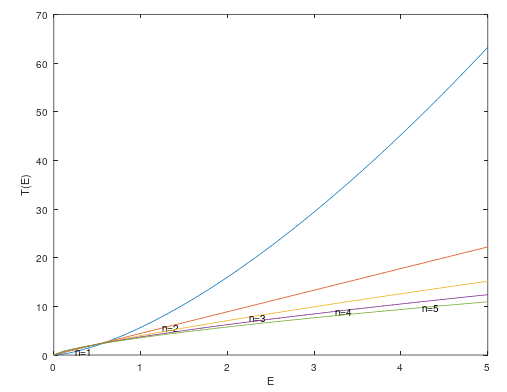
\includegraphics[width=10cm]{chapter_03_exercice_2a_result}
		\caption{$\mathrm{T}(E)$ pour $m=1$, $A=1$ et $n \in \{1,2,3,4,5\}$}\label{FIG:3_2_a_result}
	\end{center}
\end{figure}

\subsubsection{$U = -U_{0}/\cosh^{2}(\alpha x)$}

\begin{figure}[htb!]
	\begin{center}
		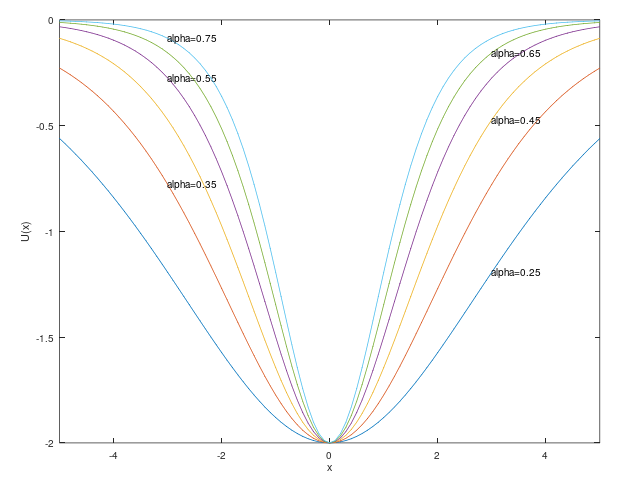
\includegraphics[width=10cm]{chapter_03_exercice_2b}
		\caption{$U = -2 / \cosh^{2}(\alpha x)$ pour $\alpha \in \{0.25,0.35,0.45,0.55,0.65,0.75\}$}\label{FIG:3_2_b}
	\end{center}
\end{figure}

\subsubsection{$U = U_{0}\tan^{2}(\alpha x)$}

\begin{figure}[htb!]
	\begin{center}
		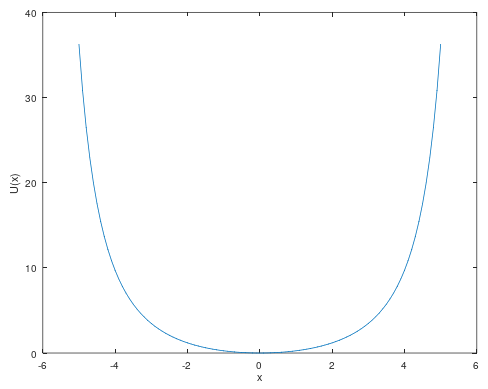
\includegraphics[width=10cm]{chapter_03_exercice_2c}
		\caption{$U = 4\tan^{2}(\alpha x)$ pour $\alpha \in \{0.25,0.35,0.45,0.55,0.65,0.75\}$}\label{FIG:3_2_c}
	\end{center}
\end{figure}